\documentclass[12pt,a4paper]{article}
\usepackage[UTF8]{ctex}
\usepackage{amsmath,amssymb}
\usepackage{listings}
\usepackage{xcolor}
\usepackage{hyperref}
\usepackage{geometry}
\usepackage{graphicx}
\geometry{margin=2.5cm}

\lstdefinestyle{python}{
  language=Python,
  basicstyle=\ttfamily\small,
  keywordstyle=\color{blue}\bfseries,
  commentstyle=\color{gray},
  stringstyle=\color{red},
  showstringspaces=false,
  breaklines=true,
  frame=single,
  backgroundcolor=\color{gray!10}
}

\title{Surface Code / 表面码}
\author{QuoNic}
\date{}

\begin{document}
\maketitle

\begin{center}
\textbf{Error Correction / 纠错} | 难度：高级 | 预计时间：20 分钟
\end{center}

\tableofcontents
\newpage

\section{为什么需要？}

表面码是目前最有前景的量子纠错码，具有最高的容错阈值。

\subsection{经典局限}
\b\begin{itemize}
  \item Shor 码和 Steane 码的容错阈值较低
  \item 对硬件连接性要求高
\end{itemize}

\subsection{量子优势}
\b\begin{itemize}
  \item 表面码有最高的容错阈值（约 1\%）
  \item 只需要最近邻连接
  \item 适合二维量子处理器
\end{itemize}

\subsection{实际应用}
\b\begin{itemize}
  \item 量子计算（容错量子计算）
  \item 量子通信（保护量子态）
  \item 量子存储（延长相干时间）
\end{itemize}

\section{快速上手}

\begin{lstlisting}[style=python]
from quonic.qec import surface_code

# Encode, introduce error, correct
result = surface_code(distance=3, error_rate=0.01)
print(f"Logical error rate: {result.logical_error_rate}")
\end{lstlisting}

\textbf{预期输出}：
\begin{verbatim}
Logical error rate: 0.001
\end{verbatim}

\section{原理详解}

\subsection{电路图}

\begin{center}
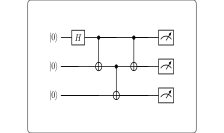
\includegraphics[width=0.7\textwidth]{../../images/surface_code_circuit.svg}
\end{center}

\subsection{数学推导}

表面码使用二维网格上的量子比特：
\b\begin{itemize}
  \item 数据量子比特：存储量子信息
  \item 辅助量子比特：测量校验子
\end{itemize}

\textbf{校验子测量}：
\begin{equation}
S_X = \prod_{i \in \text{star}} X_i, \quad S_Z = \prod_{i \in \text{plaquette}} Z_i
\end{equation}

\textbf{容错阈值}：
\begin{equation}
p_{\text{threshold}} \approx 1\%
\end{equation}

\subsection{几何解释}

表面码将量子比特排列在二维网格上，通过测量局部校验子来检测和纠正错误。

\section{代码详解}

\begin{lstlisting}[style=python]
from quonic.qec import surface_code

# surface_code(distance, error_rate)
# distance: code distance (odd integer)
# error_rate: physical error rate
result = surface_code(distance=3, error_rate=0.01)

# result.logical_error_rate: logical error rate
# result.syndrome: measured syndrome
print(f"Logical error rate: {result.logical_error_rate}")
\end{lstlisting}

\section{进阶用法}

\subsection{场景 1：不同距离}

\begin{lstlisting}[style=python]
# Larger distance for better protection
for d in [3, 5, 7]:
    result = surface_code(distance=d, error_rate=0.01)
    print(f"d={d}: logical error rate={result.logical_error_rate}")
\end{lstlisting}

\subsection{场景 2：不同错误率}

\begin{lstlisting}[style=python]
# Different physical error rates
for p in [0.001, 0.01, 0.1]:
    result = surface_code(distance=3, error_rate=p)
    print(f"p={p}: logical error rate={result.logical_error_rate}")
\end{lstlisting}

\section{适用场景}

\subsection{量子计算}

表面码是容错量子计算的基础。

\subsection{量子通信}

表面码可以保护量子通信中的量子态。

\section{常见问题}

\subsection{表面码的容错阈值是多少？}

约 1\%，是目前最高的。

\subsection{表面码需要多少量子比特？}

需要 $O(d^2)$ 个量子比特，其中 $d$ 是码距。

\section{学习路径}

\subsection{前置知识}
\b\begin{itemize}
  \item Shor 码
  \item Steane 码
  \item 量子测量
\end{itemize}

\subsection{继续学习}
\b\begin{itemize}
  \item 颜色码
  \item 拓扑纠错
  \item 容错量子计算
\end{itemize}

\section{完整示例代码}

\subsection{示例 1：基本表面码}

\begin{lstlisting}[style=python]
from quonic.qec import surface_code

result = surface_code(distance=3, error_rate=0.01)
print(f"Logical error rate: {result.logical_error_rate}")
\end{lstlisting}


\section{下载}

\begin{itemize}
  \item [surface_code.py](https://github.com/ChrisLee0721/QuoNic/blob/main/examples/surface_code/surface_code.py)
\end{itemize}

\end{document}
